\chapter{Autoencoder Implementation Details} \label{ann:AE}

\section{Generative Model Code}
Below is the implementation of the \ac{AE} model architecture used for generating images. This code defines the architecture of the encoder and decoder components, as well as the training and testing functions.

\begin{lstlisting}[language=Python, caption={Model architecture}]
class AutoEncoder(nn.Module):
    # ... (other class operations)

    def forward(self, x):
        # passes the input through the encoder and then through the decoder
        x = x.float()
        encoded = self.encoder(x)
        decoded = self.decoder(encoded)
        return decoded

    def _build_encoder(self):
        layers = []

        layers.append(nn.Conv1d(1, 32, kernel_size=9, stride=1, padding=4))
        layers.append(nn.BatchNorm1d(32))
        layers.append(nn.Tanh())
        layers.append(nn.MaxPool1d(kernel_size=2, stride=2))

        for i in range(self.convolutional_layers - 1):
            layers.append(nn.Conv1d(2**i*32, 2**(i+1)*32,
                          kernel_size=9, stride=1, padding=4))

            layers.append(nn.BatchNorm1d(2**(i+1)*32))
            layers.append(nn.Tanh())

            layers.append(nn.MaxPool1d(kernel_size=2, stride=2))

        return nn.Sequential(*layers)

    def _build_decoder(self):
        layers = []

        for i in range(self.convolutional_layers - 2, -1, -1):
            layers.append(nn.Upsample(scale_factor=2))
            layers.append(nn.ConvTranspose1d(2**(i+1)*32, 2**i *
                          32, kernel_size=9, stride=1, padding=4))
            layers.append(nn.BatchNorm1d(2**i*32))
            layers.append(nn.Tanh())

        layers.append(nn.Upsample(scale_factor=2))
        layers.append(nn.ConvTranspose1d(
            32, 1, kernel_size=9, stride=1, padding=4))
        layers.append(nn.BatchNorm1d(1))
        layers.append(nn.Tanh())

        return nn.Sequential(*layers)
\end{lstlisting}

\section{Training Code}
The following code snippet showcases the training operations for the \ac{AE} model. It includes data loading, computation of prediction error, backpropagation, and optimization.

\begin{lstlisting}[language=Python, caption={Training operations}]
def train(data_loader, model, loss_fn, optimizer):
    model.train()

    for batch, (sample, label, _) in enumerate(data_loader):
        # normalize the audio wav sample
        sample = sample / 32768

        # ... (other input operations)

        # compute prediction error
        pred = model(sample)
        loss = loss_fn(pred, sample)

        # backpropagation
        optimizer.zero_grad()
        loss.backward()
        optimizer.step()

        # ... (printing and memory management operations)


def test(data_loader, model, loss_fn, name):
    model.eval()

    test_loss, average_mse = 0, 0
    showed = False

    with torch.no_grad():
        for sample, label, _ in data_loader:
            sample = sample / 32768

            # ... (other input operations)

            pred = model(sample)
            test_loss += loss_fn(pred, sample).item()

            average_mse += torch.mean((pred - sample) ** 2)

            # ... (input operations)

    test_loss /= len(data_loader)
    average_mse /= len(data_loader)

    return test_loss, average_mse

def run():
    # model initialization
    model = AutoEncoder(convolutional_layers=4).to(device)
    loss_fn = nn.MSELoss()
    optimizer = torch.optim.Adam(model.parameters(), lr=1e-3)

    # start training
    # ... (display and early stopping initializations)
    epoch = 0

    while True: # actual code checks for early stopping
        train(dataloader_train, model, loss_fn, optimizer)
        loss, mse = test(dataloader_test, model, loss_fn, f"{conv_layers}_{epoch}")

        # ... (early stopping settings)

        epoch += 1

    # ... (printing and storing settings)
\end{lstlisting}

\section{Results}

This section presents a comparison of an original sound, represented by a soundwave, and its recreation.

It is important to note that the recreated image is the result of the original sound passing through an \ac{AE} with the specified threshold, as detailed in the accompanying annex.

This result was achieved after only 20 epochs, and the recreated sound is nearly as good as the original.

\begin{figure}[ht]
    \centering
    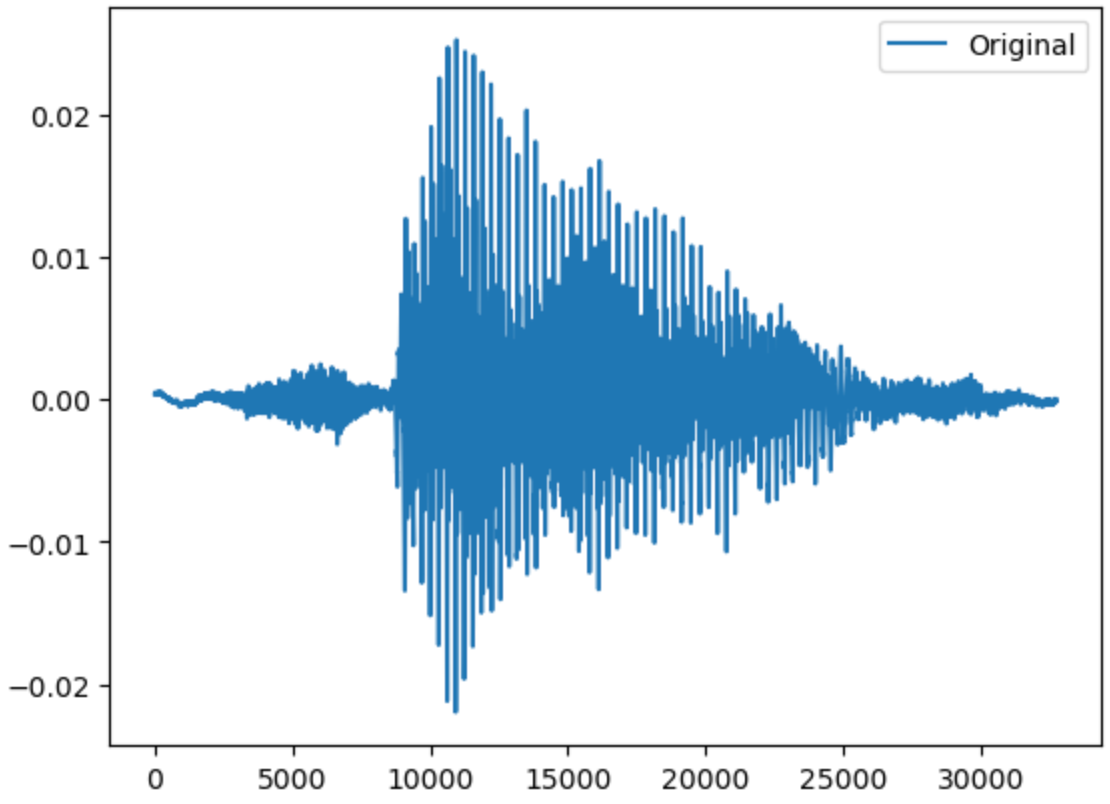
\includegraphics[width=0.7\linewidth]{annexes/AE/original.png}
    \caption{Original Sample}
\end{figure}

\begin{figure}[ht]
    \centering
    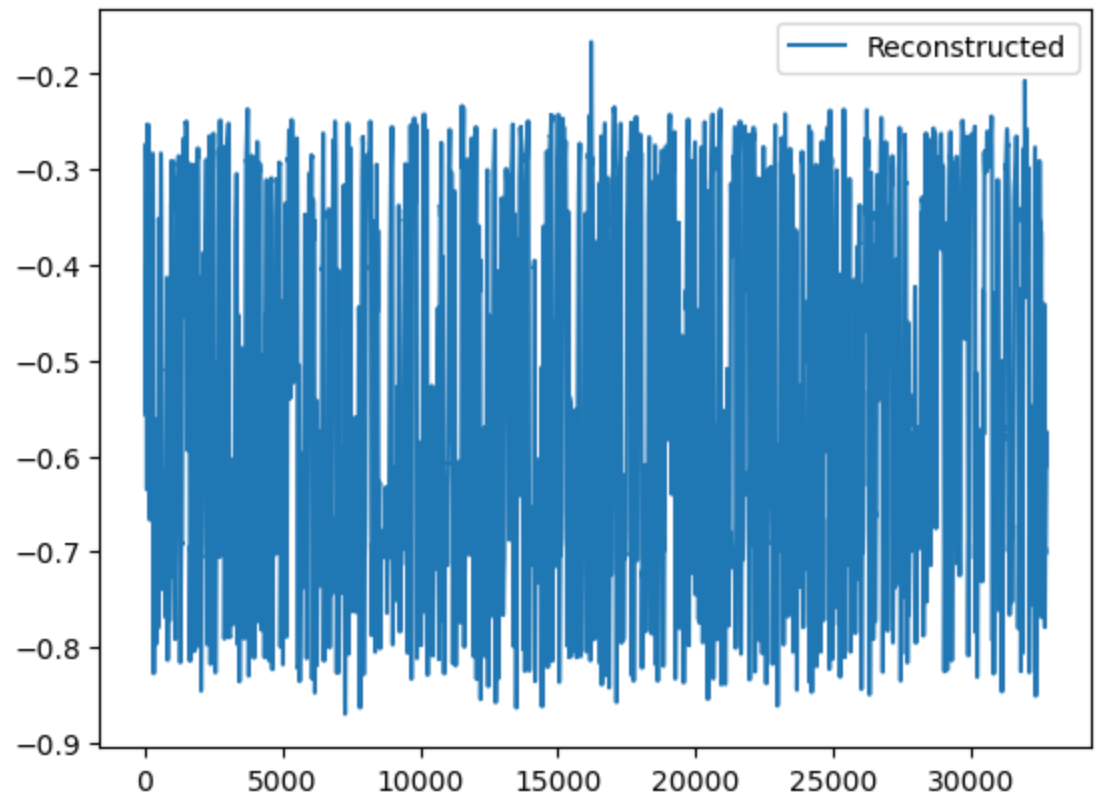
\includegraphics[width=0.7\linewidth]{annexes/AE/reconstructed.png}
    \caption{Reconstructed Sample}
\end{figure}
